%!TEX root = main.tex

\section{Charged-particle multiplicity}



\begin{frame}
\frametitle{Ch-particle multiplicity study at ALICE}
\begin{itemize}
	\item{Published multiplicity papers}
\end{itemize}
\begin{table}[htp]
\begin{center}
\begin{tabular}{|c|c|c|}
\hline
Type & $\sqrt{s}$, $\sqrt{s_\mathrm{NN}}$ (TeV) & paper\\
\hline
pp & 0.9, 2.76, 7 and 8 & Eur. Phys. J. C 77 (2017) 33\\
pp & 13 & Phys. Lett. B 753 (2016) 319-329 \\
\hline
p-Pb & 5.02 & Phys. Rev. Lett. 110 (2013) 032301 \\
\hline
Pb-Pb & 2.76 & Phys. Rev. Lett. 106, 032301 (2011) \\
Pb-Pb & 5.02 & Phys. Rev. Lett. 116 (2016) 222302 \\
\hline
\end{tabular}
\end{center}
\label{default}
\end{table}%

\begin{itemize}
	\item{Reference for all measurements in ALICE}
\end{itemize}
\begin{itemize}
	\item{Missing block}
	\begin{itemize}
		\item{pp at $\sqrt{s} = 5.02$ TeV (3 collision types comparable)}
		\item{p-Pb at $\sqrt{s_\mathrm{NN}} = 8$ TeV}
	\end{itemize}
	
\end{itemize}
\end{frame}
\setbeamerfont{footnote}{size=\tiny}

\begin{frame}
\frametitle{Ch-particle multiplicity density at $\sqrt{s}$ = 5.02 TeV}
\begin{columns}[c]
\column{.48\textwidth}
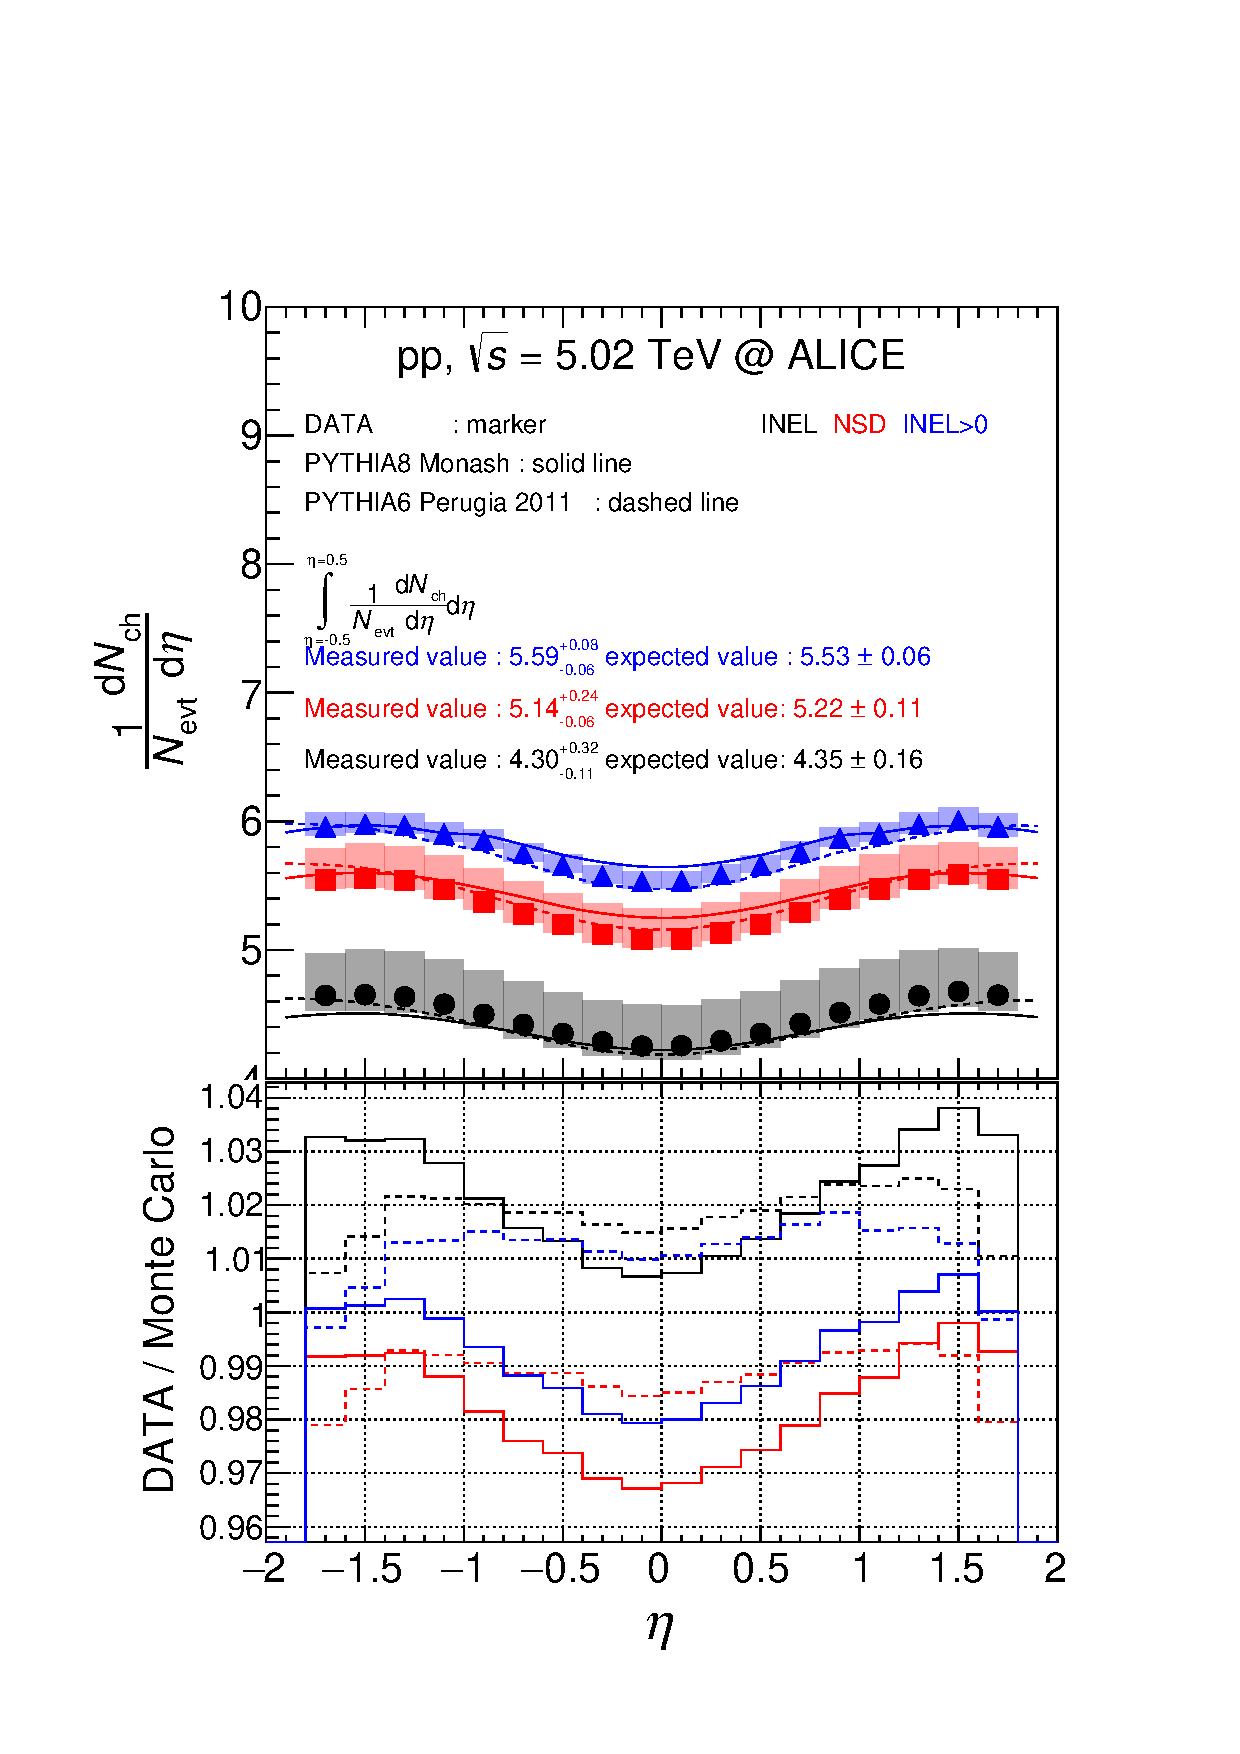
\includegraphics[width=0.93\linewidth]{../Figures/FinalResults}\\
\column{.48\textwidth}
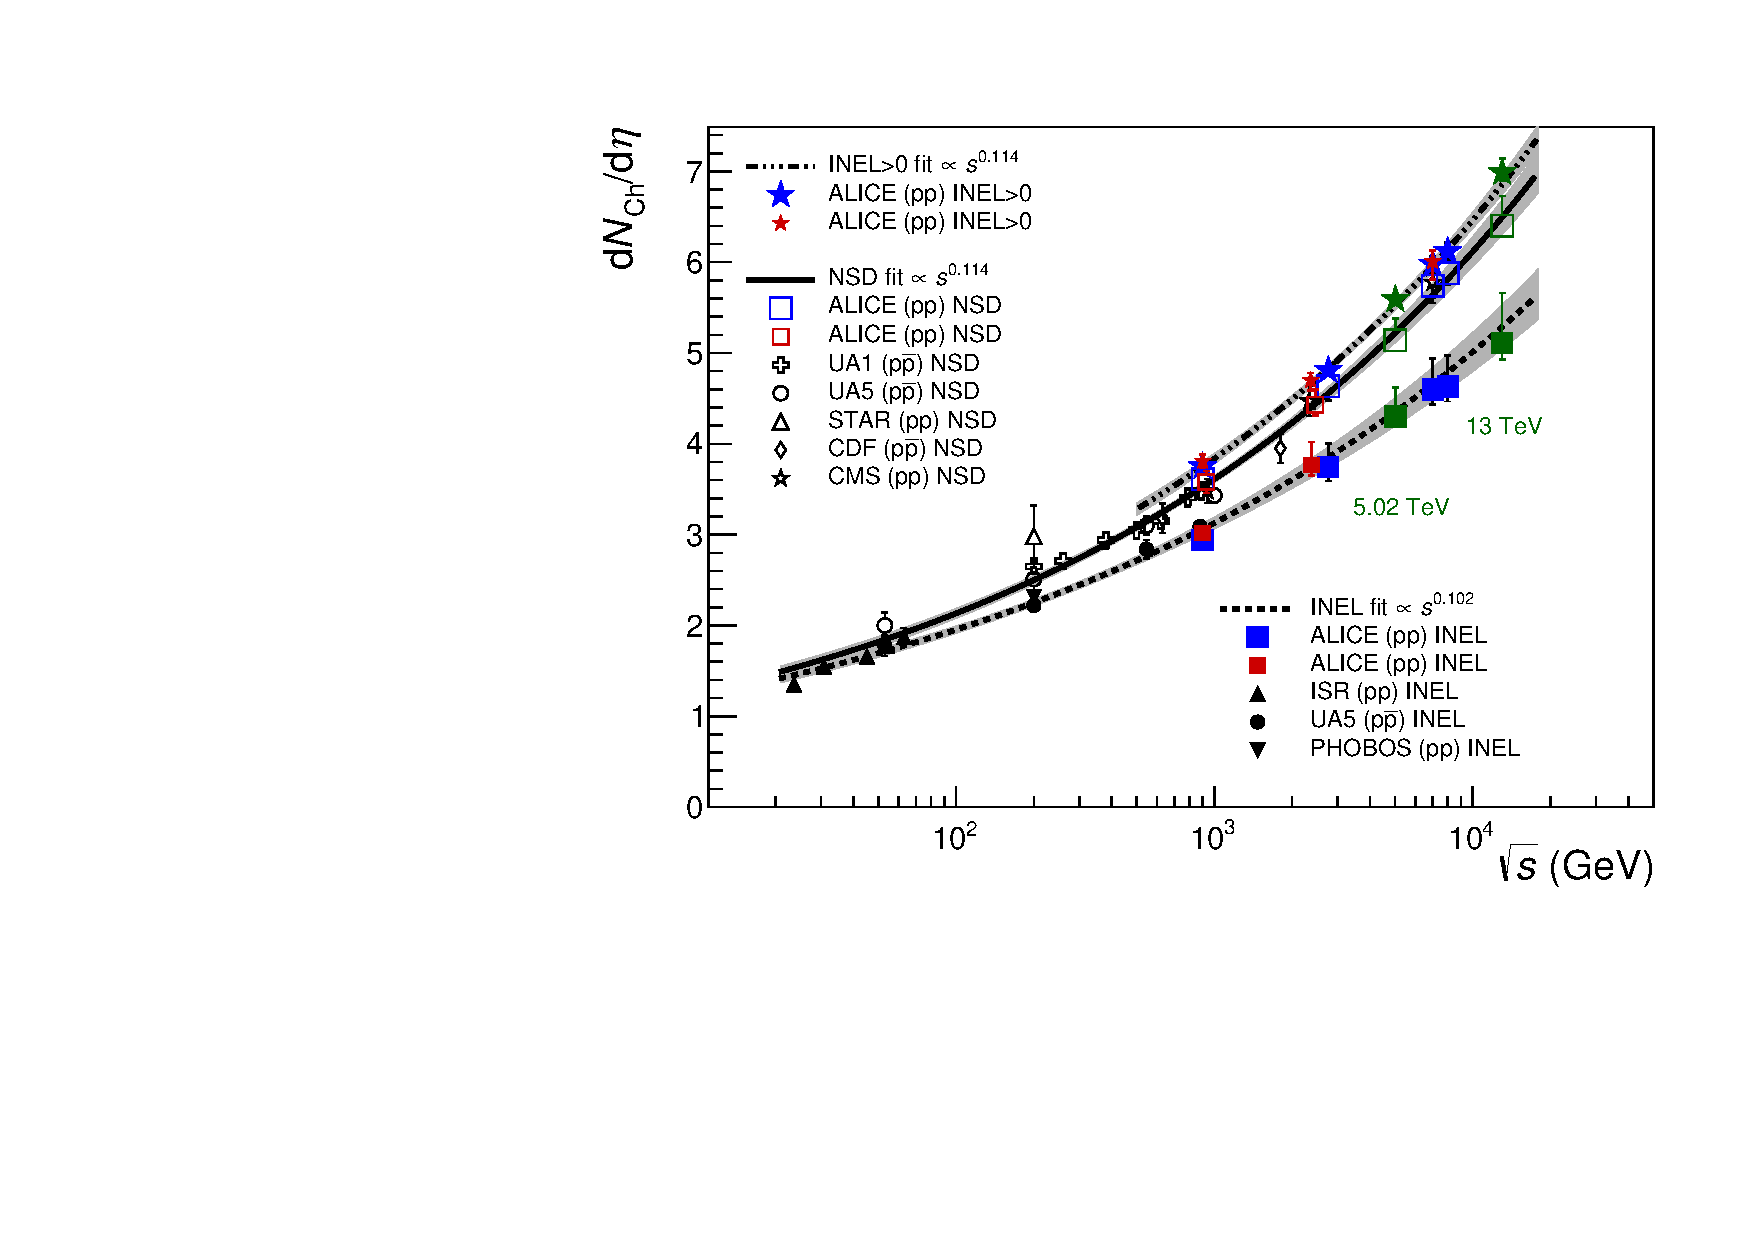
\includegraphics[width=1\linewidth]{../Figures/mulvsenergy}\\
\begin{itemize}
	\small
	\item{INEL\footnotemark[1] $\sim s^{0.102}$  }
	\item{NSD\footnotemark[2] $\sim s^{0.114}$  }  
	\item{$\mathrm{INEL>0}$\footnotemark[3] $\sim s^{0.114}$}
	\item{The power law still governs  \\(up to 13 TeV).}
\end{itemize}
\end{columns}
\footnotetext[1]{INEL = ND($\sim$ 70 $\%$) + SD ($\sim$ 20 $\%$) + DD ($\sim$ 10 $\%$) + CD ($\sim$ 1 $\%$)}
\footnotetext[2]{NSD (Non-Single Diffraction, INEL - SD) : Good event class with reduced uncertainty from SD events}
\footnotetext[3]{$\mathrm{INEL>0}$ : at least 1 ch-particle in $|\eta|<1$ to suppress SD and DD events}
\end{frame}

\begin{frame}
\frametitle{Ch-particle multiplicity density w.r.t multiplicity bin}
\begin{columns}[c]
\column{.5\textwidth}
\centering
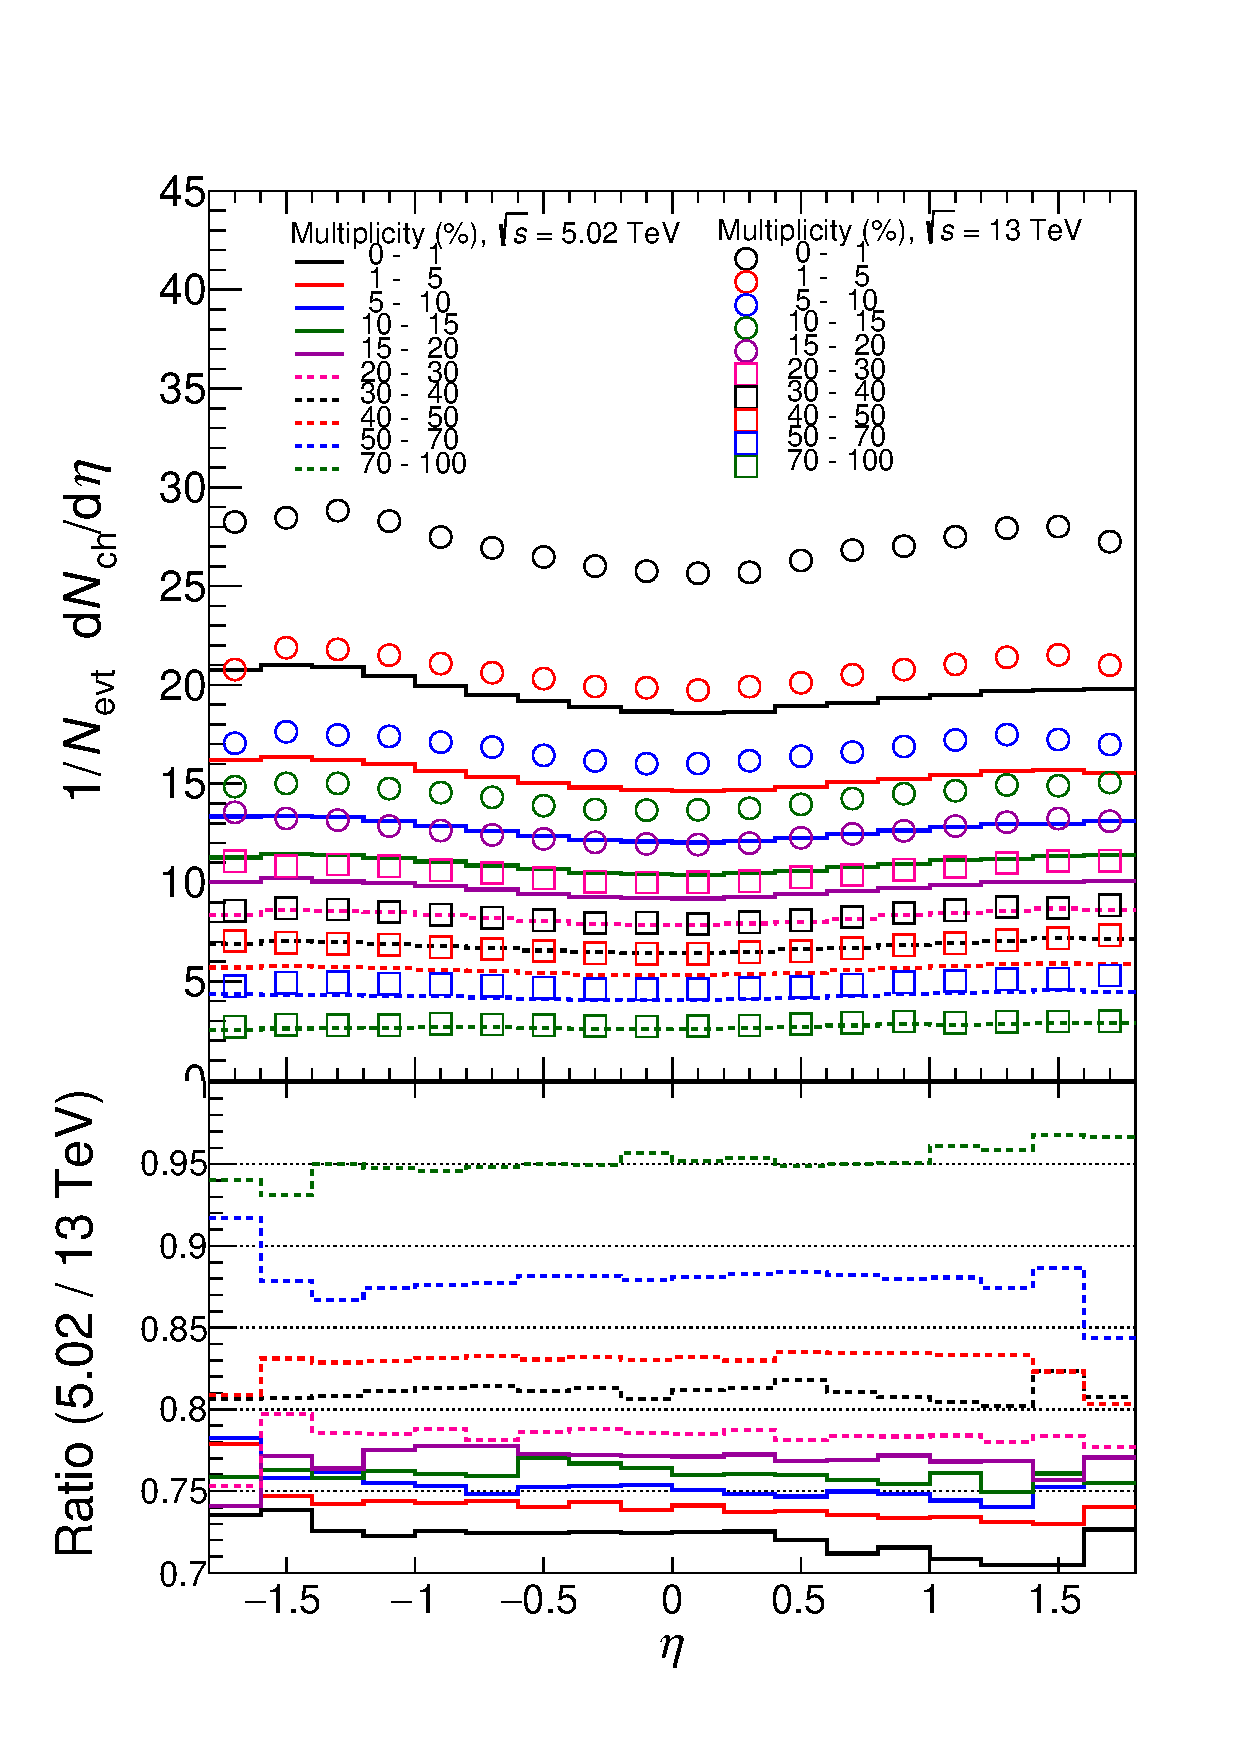
\includegraphics[width=1\linewidth]{../Figures/MultDependentResults}\\
\column{.5\textwidth}
Motivation\\
\begin{itemize}
	\item{Mid and forward ch-particle-mul correlation}
\end{itemize}
$\mathrm{d}N/\mathrm{d}\eta$ w.r.t multiplicity bin
\begin{itemize}
	\item{Study is finalizing \\for $\sqrt{s}$ = 5.02 TeV}
	\item{Cross-check \\for $\sqrt{s}$ = 13 TeV}
\end{itemize}
\end{columns}
\end{frame}

\begin{frame}
\frametitle{Ch-particle multiplicity density w.r.t multiplicity bin}
\centering
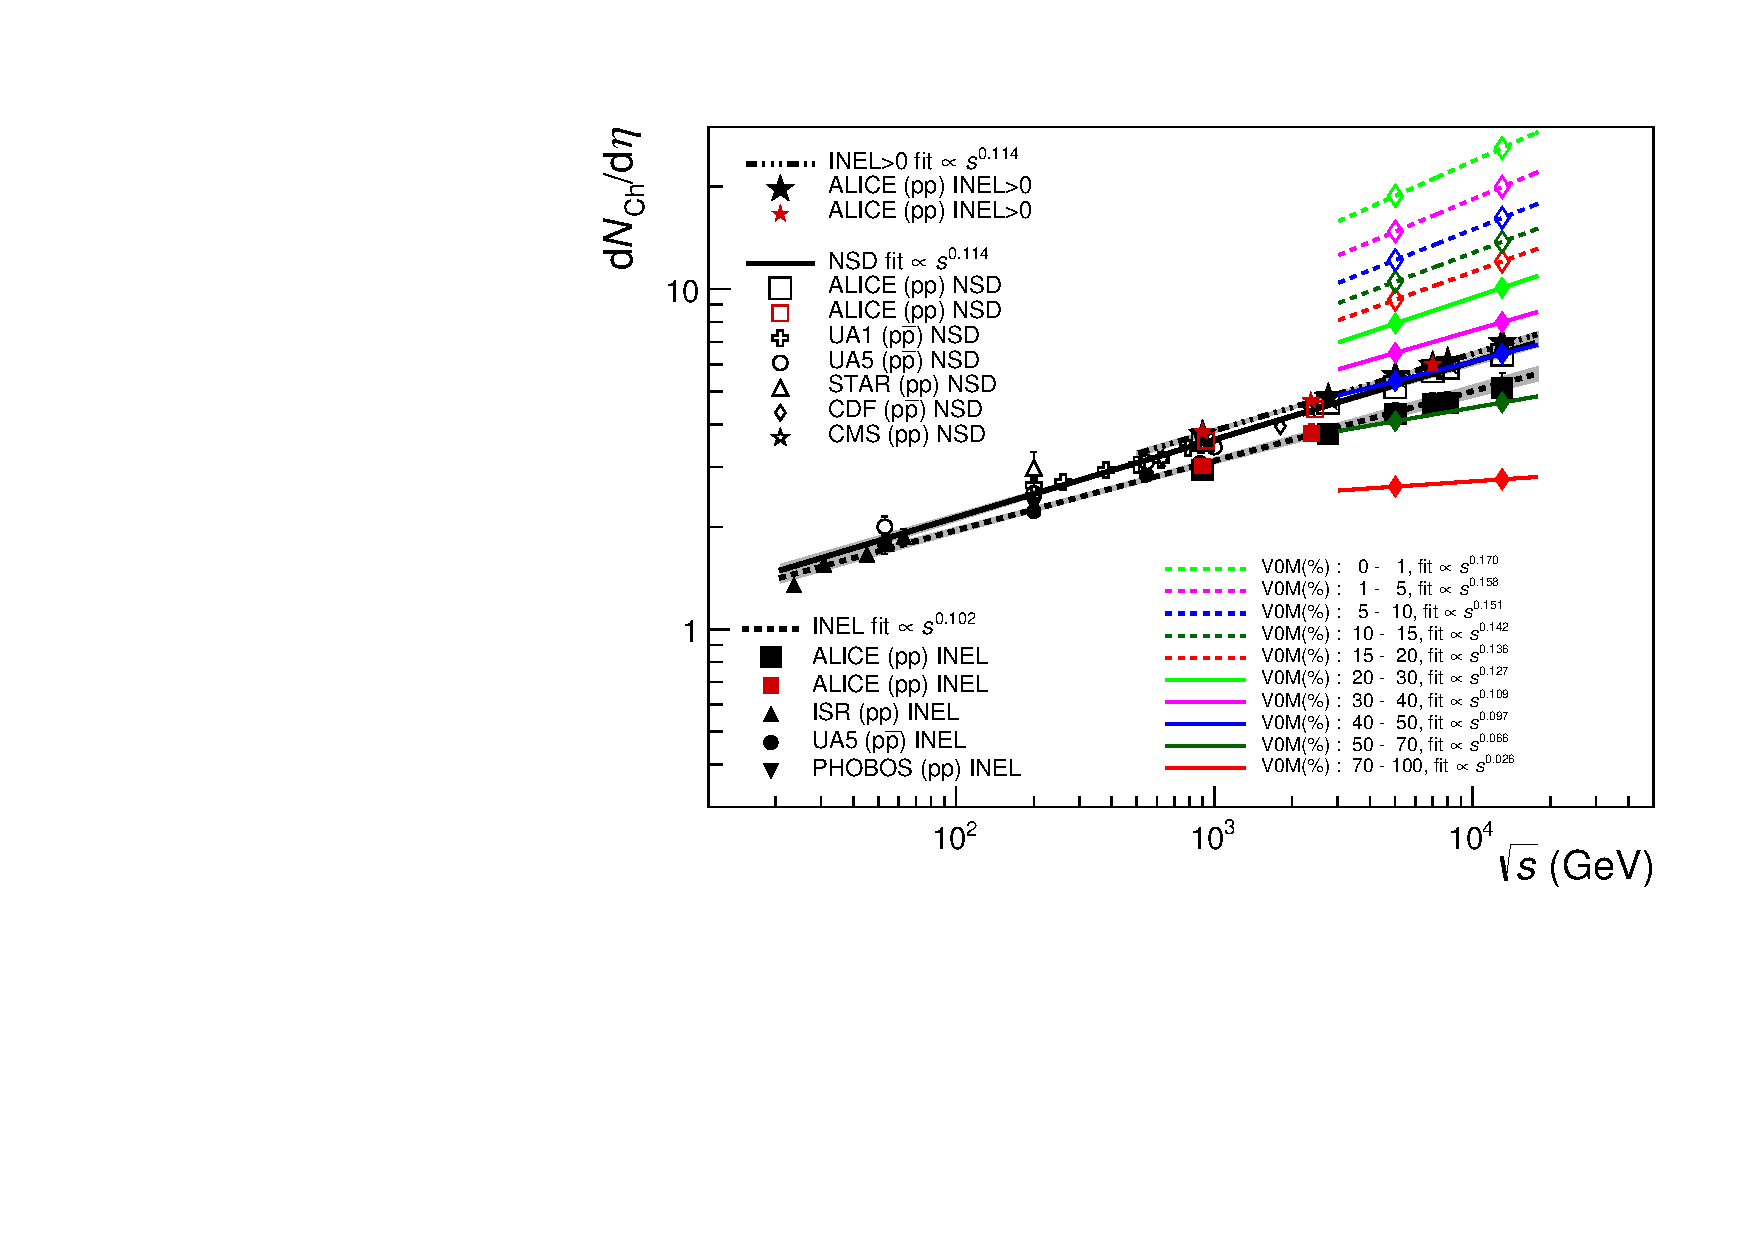
\includegraphics[width=0.9\linewidth]{../Figures/dNdeta_energy_cent}\\
Relative multiplicity density in mid increases faster \\than forward-mul density as $\sqrt{s}$ increases

\end{frame}






















